% Options for packages loaded elsewhere
\PassOptionsToPackage{unicode}{hyperref}
\PassOptionsToPackage{hyphens}{url}
\PassOptionsToPackage{dvipsnames,svgnames,x11names}{xcolor}
%
\documentclass[
  authoryear,
  preprint,
  3p]{elsarticle}

\usepackage{amsmath,amssymb}
\usepackage{lmodern}
\usepackage{iftex}
\ifPDFTeX
  \usepackage[T1]{fontenc}
  \usepackage[utf8]{inputenc}
  \usepackage{textcomp} % provide euro and other symbols
\else % if luatex or xetex
  \usepackage{unicode-math}
  \defaultfontfeatures{Scale=MatchLowercase}
  \defaultfontfeatures[\rmfamily]{Ligatures=TeX,Scale=1}
\fi
% Use upquote if available, for straight quotes in verbatim environments
\IfFileExists{upquote.sty}{\usepackage{upquote}}{}
\IfFileExists{microtype.sty}{% use microtype if available
  \usepackage[]{microtype}
  \UseMicrotypeSet[protrusion]{basicmath} % disable protrusion for tt fonts
}{}
\makeatletter
\@ifundefined{KOMAClassName}{% if non-KOMA class
  \IfFileExists{parskip.sty}{%
    \usepackage{parskip}
  }{% else
    \setlength{\parindent}{0pt}
    \setlength{\parskip}{6pt plus 2pt minus 1pt}}
}{% if KOMA class
  \KOMAoptions{parskip=half}}
\makeatother
\usepackage{xcolor}
\setlength{\emergencystretch}{3em} % prevent overfull lines
\setcounter{secnumdepth}{5}
% Make \paragraph and \subparagraph free-standing
\ifx\paragraph\undefined\else
  \let\oldparagraph\paragraph
  \renewcommand{\paragraph}[1]{\oldparagraph{#1}\mbox{}}
\fi
\ifx\subparagraph\undefined\else
  \let\oldsubparagraph\subparagraph
  \renewcommand{\subparagraph}[1]{\oldsubparagraph{#1}\mbox{}}
\fi


\providecommand{\tightlist}{%
  \setlength{\itemsep}{0pt}\setlength{\parskip}{0pt}}\usepackage{longtable,booktabs,array}
\usepackage{calc} % for calculating minipage widths
% Correct order of tables after \paragraph or \subparagraph
\usepackage{etoolbox}
\makeatletter
\patchcmd\longtable{\par}{\if@noskipsec\mbox{}\fi\par}{}{}
\makeatother
% Allow footnotes in longtable head/foot
\IfFileExists{footnotehyper.sty}{\usepackage{footnotehyper}}{\usepackage{footnote}}
\makesavenoteenv{longtable}
\usepackage{graphicx}
\makeatletter
\def\maxwidth{\ifdim\Gin@nat@width>\linewidth\linewidth\else\Gin@nat@width\fi}
\def\maxheight{\ifdim\Gin@nat@height>\textheight\textheight\else\Gin@nat@height\fi}
\makeatother
% Scale images if necessary, so that they will not overflow the page
% margins by default, and it is still possible to overwrite the defaults
% using explicit options in \includegraphics[width, height, ...]{}
\setkeys{Gin}{width=\maxwidth,height=\maxheight,keepaspectratio}
% Set default figure placement to htbp
\makeatletter
\def\fps@figure{htbp}
\makeatother

\usepackage{amsmath}
\usepackage{booktabs}
\usepackage{caption}
\usepackage{longtable}
\makeatletter
\makeatother
\makeatletter
\makeatother
\makeatletter
\@ifpackageloaded{caption}{}{\usepackage{caption}}
\AtBeginDocument{%
\ifdefined\contentsname
  \renewcommand*\contentsname{Table of contents}
\else
  \newcommand\contentsname{Table of contents}
\fi
\ifdefined\listfigurename
  \renewcommand*\listfigurename{List of Figures}
\else
  \newcommand\listfigurename{List of Figures}
\fi
\ifdefined\listtablename
  \renewcommand*\listtablename{List of Tables}
\else
  \newcommand\listtablename{List of Tables}
\fi
\ifdefined\figurename
  \renewcommand*\figurename{Figure}
\else
  \newcommand\figurename{Figure}
\fi
\ifdefined\tablename
  \renewcommand*\tablename{Table}
\else
  \newcommand\tablename{Table}
\fi
}
\@ifpackageloaded{float}{}{\usepackage{float}}
\floatstyle{ruled}
\@ifundefined{c@chapter}{\newfloat{codelisting}{h}{lop}}{\newfloat{codelisting}{h}{lop}[chapter]}
\floatname{codelisting}{Listing}
\newcommand*\listoflistings{\listof{codelisting}{List of Listings}}
\makeatother
\makeatletter
\@ifpackageloaded{caption}{}{\usepackage{caption}}
\@ifpackageloaded{subcaption}{}{\usepackage{subcaption}}
\makeatother
\makeatletter
\@ifpackageloaded{tcolorbox}{}{\usepackage[many]{tcolorbox}}
\makeatother
\makeatletter
\@ifundefined{shadecolor}{\definecolor{shadecolor}{rgb}{.97, .97, .97}}
\makeatother
\makeatletter
\makeatother
\ifLuaTeX
  \usepackage{selnolig}  % disable illegal ligatures
\fi
\usepackage[]{natbib}
\bibliographystyle{elsarticle-harv}
\IfFileExists{bookmark.sty}{\usepackage{bookmark}}{\usepackage{hyperref}}
\IfFileExists{xurl.sty}{\usepackage{xurl}}{} % add URL line breaks if available
\urlstyle{same} % disable monospaced font for URLs
\hypersetup{
  pdftitle={Clinical Phenotype and Survival Analysis in Neurodevelopmental Disorder with Microcephaly, Arthrogryposis, and Structural Brain Anomalies Due to Bi-allelic Loss of Function Variants in SMPD4},
  pdfauthor={Dean Marchiori},
  pdfkeywords={NEDMABA, SMPD4},
  colorlinks=true,
  linkcolor={blue},
  filecolor={Maroon},
  citecolor={Blue},
  urlcolor={Blue},
  pdfcreator={LaTeX via pandoc}}

\setlength{\parindent}{6pt}
\begin{document}

\begin{frontmatter}
\title{Clinical Phenotype and Survival Analysis in Neurodevelopmental
Disorder with Microcephaly, Arthrogryposis, and Structural Brain
Anomalies Due to Bi-allelic Loss of Function Variants in \emph{SMPD4}}
\author[]{Dean Marchiori%
\corref{cor1}%
}
 \ead{deanmarchiori@gmail.com} 


\cortext[cor1]{Corresponding author}

        
\begin{abstract}
A recently described, rare genetic condition known as Neurodevelopmental
Disorder with Microcephaly, Arthrogryposis, and Structural Brain
Anomalies (NEDMABA) has been identified in children with bi-allelic
loss-of-function variants in \emph{SMPD4}. The progression of this
condition is not well understood with the limited case reports described
so far exhibiting a severe and clinically diverse phenotype. A gap
exists in the understanding of associations present in the heterogenous
features of the clinical phenotype, and the expected survival
probabilities of affected individuals. This is driven in part to the
paucity of analysis-ready data on reported cases. This research aims to
collate and standardise available case reports into a common dataset, to
analyse and identify meaningful clusters in the clinical phenotype, and
to quantify the survival probability for children with NEDMABA. To
overcome the challenge of multidimensional data on very few subjects, we
employ Multiple Correspondence Analysis (MCA) as a dimension reduction
technique, which is then subject to cluster analysis and interpretation.
To account for censoring in the data Kaplan-Meier estimation is
formulated calculate patient survival time. The analysis correctly
detected the classic phenotype for this condition, as well as an
additional distinct feature-cluster relating to findings of vocal cord
paralysis, feeding dysfunction and respiratory failure. Several
additional outlying and isolated clinical features were also identified.
The survival probability for those affected was found to decline sharply
in early infancy with median survival of 150 days, but with some
surviving as long as 12.5 years. This wide range of outcomes is
provisionally associated with different variant types however this
conclusion could not be validated based on very low sample sizes. This
analysis represents the first of its kind to help describe associations
and trajectories of individuals with this newly reported condition,
despite challenges with sparse and inconsistent data. This analysis can
provide clinicians and genetic counsellors with better information to
aide in decision making and support for families with this rare
condition.
\end{abstract}





\begin{keyword}
    NEDMABA \sep 
    SMPD4
\end{keyword}
\end{frontmatter}\ifdefined\Shaded\renewenvironment{Shaded}{\begin{tcolorbox}[borderline west={3pt}{0pt}{shadecolor}, interior hidden, sharp corners, enhanced, boxrule=0pt, breakable, frame hidden]}{\end{tcolorbox}}\fi

\hypertarget{introduction}{%
\section{Introduction}\label{introduction}}

Neurodevelopment disorders are a diverse and heterogeneous group of
conditions impacting the development of the nervous system, brain
function, physical development and learning ability. A recently
identified condition known as Neurodevelopmental Disorder with
Microcephaly, Arthrogryposis, and Structural Brain Anomalies (NEDMABA)
(MIM:\href{https://omim.org/entry/618622}{618622}) has been described in
children with bi-allelic loss-of-function variants in \emph{SMPD4}
\citep{magini2019loss}. Sphingomyelinases such as \emph{SMPD4} play an
important cellular role by hydrolyzing sphingomyelin into ceramide and
phosphorylcholine. \emph{SMPD4} specifically encodes one of 4 neutral
sphinogmyelinases, nSMase3 (MIM:
\href{http://omim.org/entry/610457}{610457}). So far, less than 50 cases
of this rare disorder have been reported in the literature. Clinical
phenotype data of these cases is largely heterogeneous with severe
neurological complications and early demise a key feature. This makes
the identification, diagnosis and ongoing management of cases a
challenge for patients, their families and medical practitioners.

\citet{ravenscroft2021neurogenetic} performed a study over 190 probands
and identified a novel missense variation in SMPD4 which at the time of
whole exome sequencing was not well described in the literature. The
impacted family from Melbourne exhibited features involving
arthrogryposis multiplex congenita, complex brain malformations, small
for gestation age and hypoplasia of the corpus callosum. In two of the
three related cases were additional features of microcephaly, congenital
encephalopathy, cerebellar malformation and hypoplasia and
hypomyelination.

A detailed study by \citet{magini2019loss} involved 12 unrelated
families with 32 individuals (21 with detailed clinical information).
Presentations were of microcephaly, simplified gyral pattern of the
cortex, hypomyelination, cerebellar hypoplasia, congenital
arthrogryposis, and early fetal/postnatal demise. Despite this being the
largest cohort studied, the clinical features and survival times among
participants varied greatly. Three missense changes were noted in the
study with affected children in these families often showing a milder
presentation suggestive of possible residual function. In these cases
individuals were able to develop independent motor skills, have mild
intellectual disability and arthrogryposis without evidence of
simplified gyral patterns on brain MRI. Other patients with truncating
variants are shown to have more severe presentations, while a range of
additional significant clinical features were reported involving
dysmorphic facial features, seizure, vocal cord paralysis and hearing
impairment.

A case study from China is described in \citet{ji2022case} involving a
girl presenting in infancy with intrauterine growth restriction,
microcephaly, postnatal developmental delay, arthrogryposis,
hypertonicity, seizure, and hypomyelination on brain magnetic resonance
imaging. The authors report parallels with two cases showing the same
homozygous null variant. An individual reported in
\citet{monies2019lessons} presented with distinct symptoms of brain
atrophy and skeletal dysplasia whereas the case in
\citet{magini2019loss} with the same variant exhibited more typical
clinical features.

A recent study by \citet{bijarnia2022growth} presents the case of a
22-month old girl presenting with the typical phenotype of
neurodevelopmental delay, prenatal onset growth failure, arthrogryposis,
microcephaly and brain anomalies including severe hypomyelination,
simplified gyral pattern and hypoplasia of corpus callosum and
brainstem. Notably, there was also additional non-typical clinical
findings of nystagmus and visual impairment secondary to macular
dystrophy and retinal pigment epithelial stippling at posterior pole.

Further work to collate and analyse data relating to NEDMABA is
challenging. While \citet{magini2019loss} cataloged a detailed clinical
phenotype data set as a supplementary data set to their study, these
data are not suitable for statistical analysis as presented. Many of the
clinical features are represented as free text descriptions and a
variety of non-standard terminologies are applied between cases, making
machine interpretation of the data difficult. Other studies
\citep{ji2022case, bijarnia2022growth} present only written case reports
with some tabulated summaries. While larger studies
\citep{ravenscroft2021neurogenetic, monies2019lessons} focus more on
genetic data, with less detail included on the clinical presentation of
individuals in the cohort.

To overcome these data challenges, \citet{JSSv059i10} proposes a data
structure know as `tidy' data which organises each observation in a row,
with each feature as its own column and each value in just one cell. In
this case detailed text-based data can be transformed to high
dimensional binary indicators of key clinical features. This structure
is conducive to effective statistical analysis and integrates
deliberately with the \emph{tidyverse} \citep{tidyverse} collection of
packages for data analysis in R \citep{rbase}.

Further analysis to better describe rare genetic conditions was explored
in \citet{diaz2020phenotype} in the context of large scale
genotype-phenotype analysis. The authors argue patients with rare
disorders (often in small samples) frequently present with varied
symptoms that do not match exactly with the described phenotype. When
considering this situation of low sample size data with many features,
methods in the field of multivariate statistical analysis are commonly
deployed. Here the aim is to find substructure in the data, or a simple
representation of the multi-dimensional space. Methods, such as Multiple
Correspondence Analysis \citep{le2010multiple} are appropriate for high
dimensional data comprised of binary indicators. This technique is cited
in many studies in the application of dimension reduction and clustering
of comorbidities and phenotypes from disease
\citep{han2018cluster, costa2013use}.

In terms of patient survival, methods in statistical survival analysis
are well suited and commonly used in the field of genomics
\citep{chen2014survival}. These methods in particular provide a
mechanism for dealing with right-censoring, a common feature of clinical
studies where the clinical outcome of interest may not be known by the
end of the study period.

An open research question exists around the clinical pathway and
survival time of children exhibiting bi-allelic loss-of-function
variants in \emph{SMPD4}. With current research highlighting a diverse
and heterogeneous phenotype, the relationship and correlations between
these diverse features is not well understood. Furthermore, the survival
time of affected children has not been extensively analysed despite
early-demise featuring as a severe outcome in many cases. While a
connection has been highlighted between some missense variants and a
milder presentation with longer survival \citep{magini2019loss}, this
hypothesis has not been analysed further.

This research has three key aims. First, to collate and transform the
variety of early case reports and studies on clinical phenotype data for
this novel variant into an analysis-ready \emph{tidy} data set.
Secondly, to conduct analysis on the associations between commonly
reported clinical features. Finally, to statistically quantify the
expected survival time of children with NEDMABA based on the current
case reports.

This will be the first in-depth analysis of this novel variant, which
aims to produce statistical findings to better understand this newly
described condition. This research will assist clinicians understand the
various presentations of this challenging new condition. In addition,
genetic counselling of families with affected children will benefit from
enhanced analysis on outcomes of existing reported cases.

\hypertarget{methods}{%
\section{Methods}\label{methods}}

\hypertarget{smpd4-data-package}{%
\subsection{SMPD4 Data Package}\label{smpd4-data-package}}

The data contained in \citet{magini2019loss} ``Summary of SMPD4-Related
Clinical Phenotype'' is an excel spreadsheet tabulating each of the 21
individuals from the study with clinical details recorded. The file has
21 columns (one for each individual), and 64 rows (one for each
phenotype or clinical remark).

The data were read into \texttt{R} \citep{rbase} without any changes, so
as to preserve the reproducibility of the data transformation steps. The
data were transposed to ensure it could be presented as \emph{tidy}
formatted data \citep{JSSv059i10}. This requires each variable (clinical
phenotype) forms a column; each observation (individual) forms a row and
each type of observational unit forms a table (every cell has just one
item). This resulted in a long-formatted data set of 21 rows
(individuals) and 64 columns (clinical features). In many cases, key
clinical information was entered as free-text descriptions, which
rendered any attempt of meaningful analysis impractical
(Table~\ref{tbl-nontidy}). In these cases, the text was tokenised by
separating the list of clinical observations at each comma and forming a
binary indicator column noting its presence `1' or absence `0'
(Table~\ref{tbl-tidy}).

\hypertarget{tbl-nontidy}{}
\begin{longtable}[]{@{}
  >{\raggedright\arraybackslash}p{(\columnwidth - 4\tabcolsep) * \real{0.2083}}
  >{\raggedright\arraybackslash}p{(\columnwidth - 4\tabcolsep) * \real{0.5139}}
  >{\raggedright\arraybackslash}p{(\columnwidth - 4\tabcolsep) * \real{0.2778}}@{}}
\caption{\label{tbl-nontidy}Example of non-tidy free-text descriptions
of features}\tabularnewline
\toprule()
\begin{minipage}[b]{\linewidth}\raggedright
\end{minipage} & \begin{minipage}[b]{\linewidth}\raggedright
Family 1- Individual 1
\end{minipage} & \begin{minipage}[b]{\linewidth}\raggedright
Family 1- Individual 4
\end{minipage} \\
\midrule()
\endfirsthead
\toprule()
\begin{minipage}[b]{\linewidth}\raggedright
\end{minipage} & \begin{minipage}[b]{\linewidth}\raggedright
Family 1- Individual 1
\end{minipage} & \begin{minipage}[b]{\linewidth}\raggedright
Family 1- Individual 4
\end{minipage} \\
\midrule()
\endhead
Facial dysmorphisms & short palpebral fissures, large ears, simple
helices, smooth philtrum, thin lips, bilateral simian creases & short
palpebral fissures, receding forehead, thin upper lip \\
\bottomrule()
\end{longtable}

\hypertarget{tbl-tidy}{}
\begin{longtable}[]{@{}
  >{\raggedright\arraybackslash}p{(\columnwidth - 10\tabcolsep) * \real{0.1644}}
  >{\raggedright\arraybackslash}p{(\columnwidth - 10\tabcolsep) * \real{0.1781}}
  >{\raggedright\arraybackslash}p{(\columnwidth - 10\tabcolsep) * \real{0.1644}}
  >{\raggedright\arraybackslash}p{(\columnwidth - 10\tabcolsep) * \real{0.1644}}
  >{\raggedright\arraybackslash}p{(\columnwidth - 10\tabcolsep) * \real{0.1644}}
  >{\raggedright\arraybackslash}p{(\columnwidth - 10\tabcolsep) * \real{0.1644}}@{}}
\caption{\label{tbl-tidy}Example of tidy formatted data where
individuals are transposed into rows and text into binary
indicators}\tabularnewline
\toprule()
\begin{minipage}[b]{\linewidth}\raggedright
id
\end{minipage} & \begin{minipage}[b]{\linewidth}\raggedright
short palpebral fissures
\end{minipage} & \begin{minipage}[b]{\linewidth}\raggedright
large ears
\end{minipage} & \begin{minipage}[b]{\linewidth}\raggedright
simple helices
\end{minipage} & \begin{minipage}[b]{\linewidth}\raggedright
receding forehead
\end{minipage} & \begin{minipage}[b]{\linewidth}\raggedright
\ldots{}
\end{minipage} \\
\midrule()
\endfirsthead
\toprule()
\begin{minipage}[b]{\linewidth}\raggedright
id
\end{minipage} & \begin{minipage}[b]{\linewidth}\raggedright
short palpebral fissures
\end{minipage} & \begin{minipage}[b]{\linewidth}\raggedright
large ears
\end{minipage} & \begin{minipage}[b]{\linewidth}\raggedright
simple helices
\end{minipage} & \begin{minipage}[b]{\linewidth}\raggedright
receding forehead
\end{minipage} & \begin{minipage}[b]{\linewidth}\raggedright
\ldots{}
\end{minipage} \\
\midrule()
\endhead
Family 1- Individual 1 & 1 & 1 & 1 & 0 & \ldots{} \\
Family 1- Individual 4 & 1 & 0 & 0 & 1 & \ldots{} \\
\bottomrule()
\end{longtable}

In the case where synonymous terms are present, these indicator columns
are consolidated and merged into one indicator column to prevent
duplication e.g.~\{bilateral\_cleft\_lips, bilateral\_cleft\_lip,
cleft\_lip\_b\_l\} -\textgreater{} \{bilateral\_cleft\_lip\}.

Data type conversion and categorical level standardisation was performed
to ensure the data were in consistent and appropriate data types. For
example, `Gender' was not consistently coded, and `Birth Weight' was
encoded as a text string rather than a more useful numeric format.
(Table~\ref{tbl-data-types}).

\hypertarget{tbl-data-types}{}
\begin{longtable}[]{@{}ll@{}}
\caption{\label{tbl-data-types}Example of inconsistent coding or
sub-optimal data types}\tabularnewline
\toprule()
Gender & Birth Weight \\
\midrule()
\endfirsthead
\toprule()
Gender & Birth Weight \\
\midrule()
\endhead
male & 2175 grams (- 2.5 SD) \\
female & 2045 g (-3 SD) \\
Female & 2300 gram (-2 SD) \\
Female fetus & n.a. \\
\bottomrule()
\end{longtable}

\hypertarget{tbl-data-types2}{}
\begin{longtable}[]{@{}ll@{}}
\caption{\label{tbl-data-types2}Example of consistent and appropriate
coding or data types}\tabularnewline
\toprule()
Gender & Birth Weight (g) \\
\midrule()
\endfirsthead
\toprule()
Gender & Birth Weight (g) \\
\midrule()
\endhead
male & 2175 \\
female & 2045 \\
female & 2300 \\
female & NA \\
\bottomrule()
\end{longtable}

This format was used as a template to align other written case reports
identified in the literature
\citep{ravenscroft2021neurogenetic, monies2019lessons, bijarnia2022growth, ji2022case}.
These were manually entered to conform to this template to allow the
data to be combined for further analysis.

The final data set consisted of 28 observations (one per individual) and
152 variables (one per clinical feature). These variables were comprised
of qualitative text descriptions, binary indicators of features as
described above and other fields including background information on the
patient and various bio markers. A full list of this data set is
available in Table~\ref{tbl-dict}. These data sets were compiled into a
publicly available \texttt{R} Package called \texttt{SMPD4}
\citep{smpd4-data} in order to allow for reproducibility and sharing.

\hypertarget{multiple-correspondence-analysis}{%
\subsection{Multiple Correspondence
Analysis}\label{multiple-correspondence-analysis}}

The data on subjects introduced above is subset to include only
variables that can be transformed into binary indicator variables that
represent the presence or absence of a given clinical feature. Only
those features that appeared in more than one case report were included
to minimise the influence of isolated features in this analysis.

Dimension reduction on this wide data set was performed using Multiple
Correspondence Analysis (MCA) (an analogy to Principle Component
Analysis (PCA) for categorical data) \citep{le2010multiple} in order to
arrive at a set of meaningfully small dimensions that account for most
of the variation in the data. This computation was carried out using the
\emph{FactoMineR} R package \citep{factominer}.

We let these data be \(\mathbf{X}\) which is comprised of a set of
individuals \(I\) and a set of features \(Q\) such that the \(q_{th}\)
feature has \(K_q\) levels. The sum of all categories
\(K = \sum_{q=1}^{Q}K_q\) defines the dimensionality of \(\mathbf{X}\)
as an \(I\times K\) matrix. This resulted in a data set
\(X_{28 \times 61}\) indicator matrix of 61 clinical features across 28
individuals. Taking \(\delta_{ik} = 1\) if subject \(i\) has feature
\(k\) and \(\delta_{ik} = 0\) if the subject does not, we are left with
the completely disjunctive table \(\mathbf{X} = I\times K\) of
\(\{0,1\}\). Letting the sum of all entries of \(\mathbf{X}\) be \(N\),
we have \(\mathbf{Z} = N^{-1}\mathbf{X}\). We can introduce two diagonal
matrices \(\mathbf{D_r} = diag(\mathbf{r})\) and
\(\mathbf{D_c} = diag(\mathbf{c})\) where \(\mathbf{r}\) and
\(\mathbf{c}\) are the vectors of row sums and column sums of
\(\mathbf{Z}\) respectively.

Computing MCA involves taking the Singular Value Decomposition:

\[
\mathbf{M = D_r^{-\frac{1}{2}}(Z-rc^T)D_c^{-\frac{1}{2}}} = \mathbf{P}\Delta\mathbf{Q^T}
\] where \(\Delta\) are the singular values and \(\Lambda = \Delta^2\)
is the matrix of eigenvalues.

This results in the row and column factor scores respectively as:

\[
\begin{split}
\mathbf{F} = \mathbf{D_r^{-\frac{1}{2}}P}\Delta \\
\mathbf{G = D_c^{-\frac{1}{2}}Q}\Delta
\end{split}
\]

The \emph{contribution} of each category was computed for each of the
principal axis per \citet{le2010multiple}. This metric identifies the
proportion of variance of that axis due to the point and is defined as:

\[
Ctr_k = \frac{py_k^2}{\lambda}
\] Where \(p\) represents the point weighting, \(y\) is the coordinate
relative to the principal axes of variance \(\lambda\).

The coordinates on the first few principal axes were inspected for any
outliers or unusual data before being graphically interpreted and
subject to further analysis.

\hypertarget{cluster-analysis}{%
\subsection{Cluster Analysis}\label{cluster-analysis}}

The MCA coordinates for the first 4 principal dimensions were subject to
clustering in order to find groups of features that were internally
homogeneous and externally heterogeneous. This was computed in
\texttt{R} using the \texttt{clValid} package \citep{clvalid}.

A range of clustering algorithms were compared including AGNES
hierarchical agglomerative \citep{kaufman2009finding}, k-means
\citep{hartigan1979algorithm} and self-organising maps (SOM)
\citep{kohonen2012self}. A sensible range of clusters from 2-5 were
trialed for each clustering algorithm. The results for each method were
evaluated using three measures of stability: Average proportion of
non-overlap (APN), Average Distance (AD) and Average Distance Between
Means (ADM) \citep{datta2003comparisons}. Stability measures compare the
full clustering result with a result based on dropping each of the
columns one at a time. These metrics were selected to represent each
data point (clinical feature) with a number of MCA dimensions. A good
cluster solution is one that is robust and meaningful across all of
these dimensions (Figure~\ref{fig-clvalid}). The optimal method and
cluster number was selected based on a trade off between the best
performing method using the evaluation metrics and a sensible
partitioning of the data for this analysis (Table~\ref{tbl-eig}).

\hypertarget{survival-analysis}{%
\subsection{Survival Analysis}\label{survival-analysis}}

To model survival probability for all subjects in the combined data, the
data were subsetted to include \emph{survival\_time} which is either the
number of days the individual survived for, or the age in days at last
follow up, and \emph{deceased} a numeric event indicator which is equal
to 1 if the subject is deceased and 0 if the subject was still alive at
the time the respective study had concluded. The Kaplan-Meier estimator
\citep{kaplan1958nonparametric} was used to estimate the survival
function of the data.

The estimator is calculated as:

\[
\hat{S}(t) = \prod_{t_i \leq t}\frac{n_i - d_i}{n_i} 
\] where \(t_i\) is some event time, \(d_i\) represents the number of
events (here deceased subjects) and \(n_i\) indicating the individuals
known to have survived up to \(t_i\)

The baseline estimator of all individuals was calculated using the
\emph{survival} package in \texttt{R} \citep{survival-book}. Next the
Kaplan-Meier estimator was stratified by the type of genetic variation
reported in the literature. A log-rank test was performed to detect
differences in the survival curves using methods from
\citet{harrington1982class}, again implemented in the \emph{survival}
\texttt{R} package.

\hypertarget{results}{%
\section{Results}\label{results}}

\hypertarget{mca}{%
\subsection{MCA}\label{mca}}

The initial results of the MCA were inspected with a bi-plot and
identified two subjects (17, 18) from the data that were clear outliers
and sat significantly beyond the 95\% confidence ellipse
(Figure~\ref{fig-biplotprelim}). These individuals represented two twins
from \citet{magini2019loss} who were described with a much milder
phenotype and were subject to a missense variation in \emph{SMPD4}.
Further analysis of this influence is conducted below. For now, these
subjects were removed to allow for more meaningful analysis of other
features.

Repeating MCA for the remaining subjects shows the first dimension
(\(\lambda_1 = 0.18\)) accounts for 17.88\% of the variance in the data
with the first 4 dimensions of the MCA analysis accounting for 54\% of
the variance (Table~\ref{tbl-eig}).

\begin{figure}

{\centering 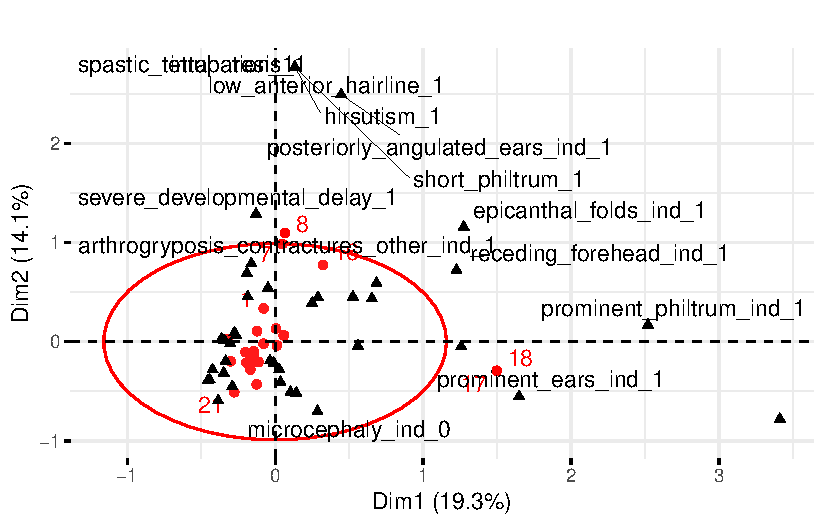
\includegraphics{paper_files/figure-pdf/fig-biplotprelim-1.pdf}

}

\caption{\label{fig-biplotprelim}A bi-plot of the first two principal
axes with grey circles indicating the individual's projected position
and black triangles indicating the variables. A 95\% confidence ellipse
is plotted in red around the origin.}

\end{figure}

\hypertarget{tbl-eig}{}
\begin{longtable}{lrrr}
\caption{\label{tbl-eig}Eigenvalues and percentage of variance explained by the MCA principal
axes }\tabularnewline

\toprule
dimension & eigenvalue & percentage of variance & cumulative percentage of variance \\ 
\midrule
dim 1 & $0.18$ & $17.88\%$ & $17.88\%$ \\ 
dim 2 & $0.14$ & $13.81\%$ & $31.70\%$ \\ 
dim 3 & $0.12$ & $12.32\%$ & $44.01\%$ \\ 
dim 4 & $0.10$ & $9.66\%$ & $53.67\%$ \\ 
dim 5 & $0.07$ & $7.49\%$ & $61.16\%$ \\ 
dim 6 & $0.06$ & $5.97\%$ & $67.13\%$ \\ 
dim 7 & $0.05$ & $4.90\%$ & $72.03\%$ \\ 
dim 8 & $0.04$ & $4.20\%$ & $76.23\%$ \\ 
dim 9 & $0.04$ & $4.08\%$ & $80.31\%$ \\ 
dim 10 & $0.03$ & $3.47\%$ & $83.78\%$ \\ 
dim 11 & $0.03$ & $2.92\%$ & $86.70\%$ \\ 
dim 12 & $0.02$ & $2.49\%$ & $89.20\%$ \\ 
dim 13 & $0.02$ & $2.15\%$ & $91.34\%$ \\ 
dim 14 & $0.02$ & $1.82\%$ & $93.16\%$ \\ 
dim 15 & $0.02$ & $1.65\%$ & $94.81\%$ \\ 
dim 16 & $0.01$ & $1.12\%$ & $95.93\%$ \\ 
dim 17 & $0.01$ & $1.00\%$ & $96.93\%$ \\ 
dim 18 & $0.01$ & $0.93\%$ & $97.85\%$ \\ 
dim 19 & $0.01$ & $0.67\%$ & $98.53\%$ \\ 
dim 20 & $0.01$ & $0.63\%$ & $99.16\%$ \\ 
dim 21 & $0.00$ & $0.41\%$ & $99.57\%$ \\ 
dim 22 & $0.00$ & $0.31\%$ & $99.88\%$ \\ 
dim 23 & $0.00$ & $0.12\%$ & $100.00\%$ \\ 
dim 24 & $0.00$ & $0.00\%$ & $100.00\%$ \\ 
dim 25 & $0.00$ & $0.00\%$ & $100.00\%$ \\ 
\bottomrule
\end{longtable}

The \emph{contribution} of the categories were ranked within each of the
first four principal dimensions in Figure~\ref{fig-ctr}. The first
dimension is dominated by isolated cases with highly specific facial
dysmorphisms such as epicanthal folds, short philtrum and low anterior
hairline. The second MCA dimension is categorised by feeding and
respiratory dysfunction with vocal cord palsy, tracheostomy, tube
feeding and GERD. Examining the bi-plot of the first two principal axes
(Figure~\ref{fig-biplot}) illustrates the contrasting sources of
variation between conditions relating to airway and swallowing function
and predominantly facial features and structural brain anomalies such as
as cerebellar hypoplasia, development delay. The third dimension is
characterised by atypical, complex features such as patent ductus
arteriosus, respiratory infections, small for gestational age and
further facial features. These are contrasted by the fourth principal
dimension which is strongly categorised by respiratory distress
including stridor and hypercapnia in the absence of typical
presentations of simplified gyral pattern, intrauterine growth
retardation and microcephaly.

\begin{figure}

{\centering 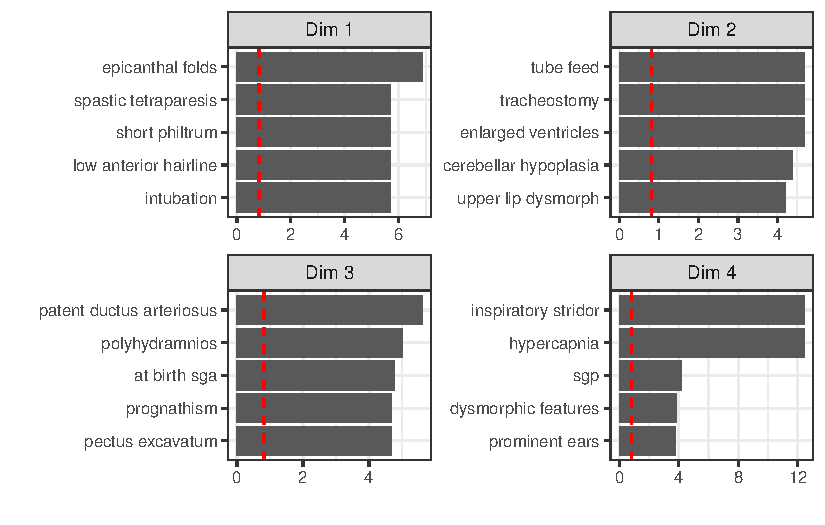
\includegraphics{paper_files/figure-pdf/fig-ctr-1.pdf}

}

\caption{\label{fig-ctr}Top 10 feature categories from MCA analysis for
the first four MCA dimensions. The red dashed line indicates the mean
contribution value. Each feature may be present or absent as indicated
by 1 or 0 respectively}

\end{figure}

\begin{figure}

{\centering 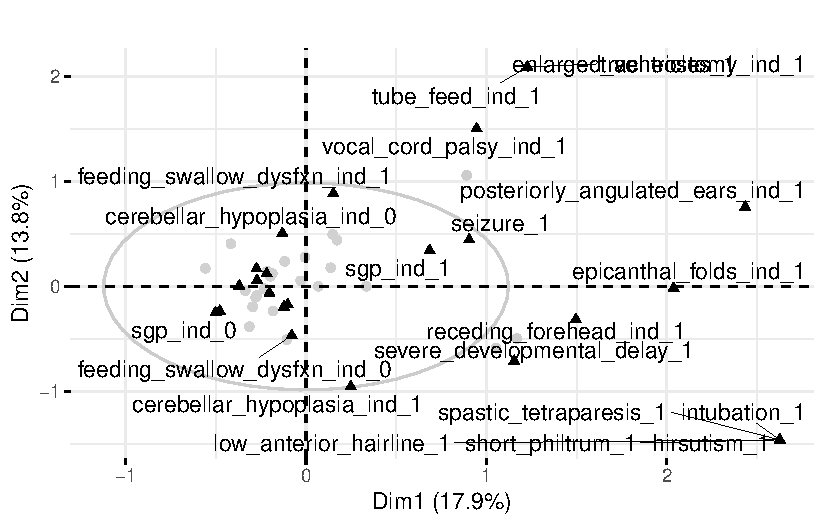
\includegraphics{paper_files/figure-pdf/fig-biplot-1.pdf}

}

\caption{\label{fig-biplot}A bi-plot of the first two principal axes
with grey circles indicating the individual's projected position and
black triangles indicating the variables. A 95\% confidence ellipse is
plotted in grey around the origin.}

\end{figure}

\begin{figure}

{\centering 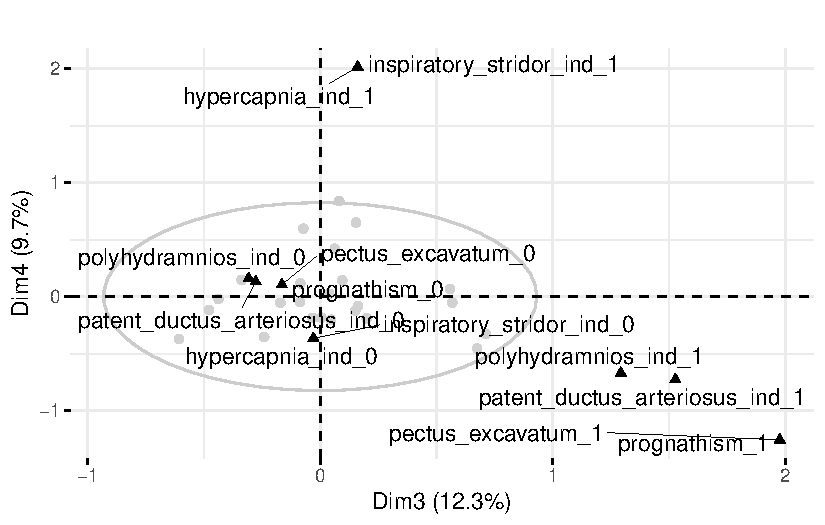
\includegraphics{paper_files/figure-pdf/fig-biplot2-1.pdf}

}

\caption{\label{fig-biplot2}A bi-plot of principal axes 3 and 4, with
grey circles indicating the individual's projected position and black
triangles indicating the variables. A 95\% confidence ellipse is plotted
in grey around the origin.}

\end{figure}

\hypertarget{cluster-analysis-1}{%
\subsection{Cluster Analysis}\label{cluster-analysis-1}}

Cluster validation measures resulted in either 2 or 5 clusters as the
optimal choice (Table~\ref{tbl-opticlust}). In order to partition the
data into meaningful groupings, k-means with 5 clusters was selected.
This reflects the optimal choice for both AD and FOM cluster metrics. A
scatter plot of the cluster results shown in Figure~\ref{fig-clust} is
projected on the first two principal dimensions highlights a core
cluster of classic features of NEDMABA such as microcephaly,
hypomyelination, arthrogryposis and feet deformity and structural brain
anomalies. A separate and adjacent cluster is formed of airway and
feeding related conditions involving vocal cord paralysis, tracheostomy,
tube feeding and enlarged ventricles. Three other smaller satellite
clusters exists where highly distinctive features were associated with a
single individual or family. A full articulation of feature to cluster
assignment is given in Table~\ref{tbl-profile}.

\hypertarget{tbl-opticlust}{}
\begin{longtable}{lrlr}
\caption{\label{tbl-opticlust}Optimal clusters }\tabularnewline

\toprule
Metric & Score & Method & Clusters \\ 
\midrule
APN & $0.07$ & agnes & 2 \\ 
AD & $1.38$ & kmeans & 5 \\ 
ADM & $0.33$ & kmeans & 2 \\ 
FOM & $0.65$ & kmeans & 5 \\ 
\bottomrule
\end{longtable}

\begin{figure}

{\centering 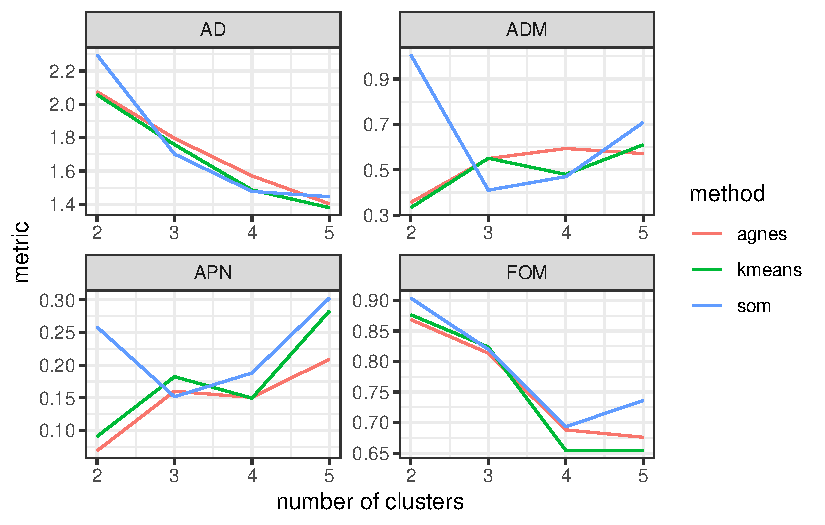
\includegraphics{paper_files/figure-pdf/fig-clvalid-1.pdf}

}

\caption{\label{fig-clvalid}cluster validation analysis showing various
metrics for cluster evaluation from 2 to 5 clusters. The most optimal
number of clusters are selected by picking the lowest value from one or
many of these comparable metrics.}

\end{figure}

\begin{figure}

{\centering 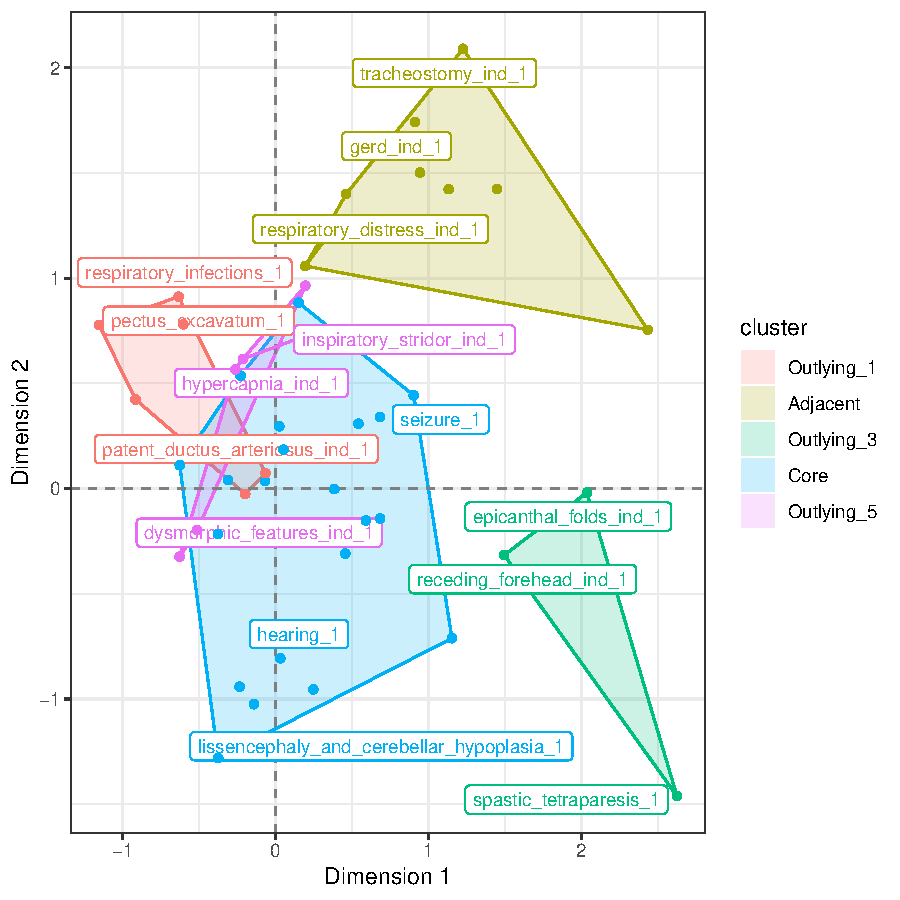
\includegraphics{paper_files/figure-pdf/fig-clust-1.pdf}

}

\caption{\label{fig-clust}A projection of features on the first two
principal components with k-means cluster assignment indicated by
colour. A random sample of three labels per cluster are printed to
provide a representation of each cluster's characteristics.}

\end{figure}

\hypertarget{survival-analysis-1}{%
\subsection{Survival Analysis}\label{survival-analysis-1}}

The Kaplan-Meier estimator shows a range of survival times (0, 4562
days) with median survival time calculated as 150 days. At time 0 the
survival probability was 0.82 (95\% CI: 0.69, 0.98). Survival
probability after one year at 0.403 (95\% CI: 0.252, 0.644) and survival
probability at close to ten years of 0.24 (95\% CI: 0.11, 0.52).

\begin{longtable}[]{@{}rrrrrrrr@{}}
\caption{Survival probabilities derived from Kaplan-Meier estimation for
the range of recorded survival times, including 95\% Confidence
Interval.}\tabularnewline
\toprule()
time & n.risk & n.event & n.censor & surv & std.err & upper & lower \\
\midrule()
\endfirsthead
\toprule()
time & n.risk & n.event & n.censor & surv & std.err & upper & lower \\
\midrule()
\endhead
0.0 & 28 & 5 & 0 & 0.82 & 0.09 & 0.98 & 0.69 \\
15.0 & 23 & 1 & 0 & 0.79 & 0.10 & 0.95 & 0.65 \\
30.0 & 22 & 2 & 0 & 0.71 & 0.12 & 0.90 & 0.57 \\
47.0 & 20 & 1 & 0 & 0.68 & 0.13 & 0.88 & 0.53 \\
60.0 & 19 & 1 & 1 & 0.64 & 0.14 & 0.85 & 0.49 \\
67.0 & 17 & 1 & 0 & 0.61 & 0.15 & 0.82 & 0.45 \\
90.0 & 16 & 0 & 1 & 0.61 & 0.15 & 0.82 & 0.45 \\
120.0 & 15 & 2 & 0 & 0.52 & 0.18 & 0.75 & 0.37 \\
150.0 & 13 & 1 & 0 & 0.48 & 0.20 & 0.72 & 0.33 \\
180.0 & 12 & 1 & 0 & 0.44 & 0.22 & 0.68 & 0.29 \\
240.0 & 11 & 1 & 0 & 0.40 & 0.24 & 0.64 & 0.25 \\
270.0 & 10 & 0 & 1 & 0.40 & 0.24 & 0.64 & 0.25 \\
365.0 & 9 & 0 & 1 & 0.40 & 0.24 & 0.64 & 0.25 \\
750.0 & 8 & 1 & 0 & 0.35 & 0.27 & 0.60 & 0.21 \\
1095.0 & 7 & 1 & 0 & 0.30 & 0.31 & 0.56 & 0.16 \\
1825.0 & 6 & 0 & 1 & 0.30 & 0.31 & 0.56 & 0.16 \\
2190.0 & 5 & 1 & 0 & 0.24 & 0.39 & 0.52 & 0.11 \\
3285.0 & 4 & 0 & 2 & 0.24 & 0.39 & 0.52 & 0.11 \\
4380.0 & 2 & 1 & 0 & 0.12 & 0.81 & 0.59 & 0.02 \\
4562.5 & 1 & 1 & 0 & 0.00 & Inf & NA & NA \\
\bottomrule()
\end{longtable}

\begin{figure}

{\centering 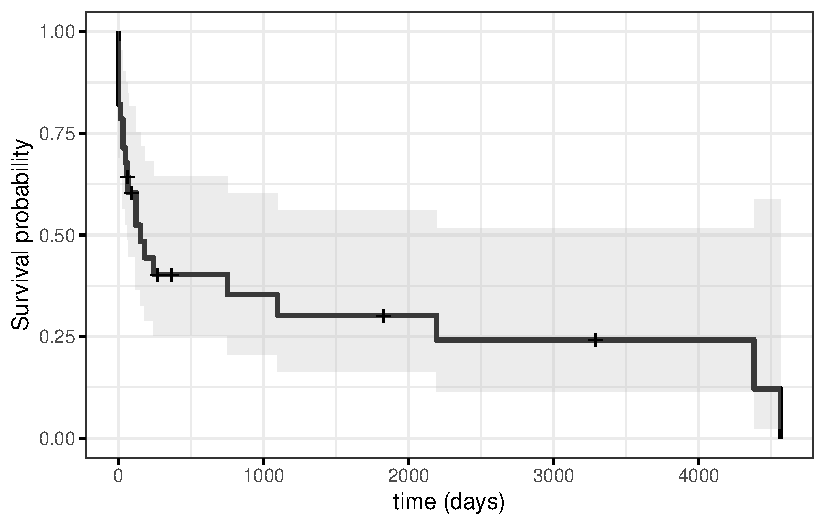
\includegraphics{paper_files/figure-pdf/fig-surv-1.pdf}

}

\caption{\label{fig-surv}Kaplan Meier curve with the black line
representing the survival probability and with grey shading indicating
the 95\% confidence interval. Cross icons represent right-censoring}

\end{figure}

A comparative box plot of survival times by variant type shows
significant outliers for compound heterozygous \emph{missense + splice}
and homozygous \emph{missense} variants. However, even within homozygous
missense variants the survival time varies greatly. Other missense
variants, such as heterozygous missense with gene deletion do not show
the same increased survival time as noted by \citet{magini2019loss}.

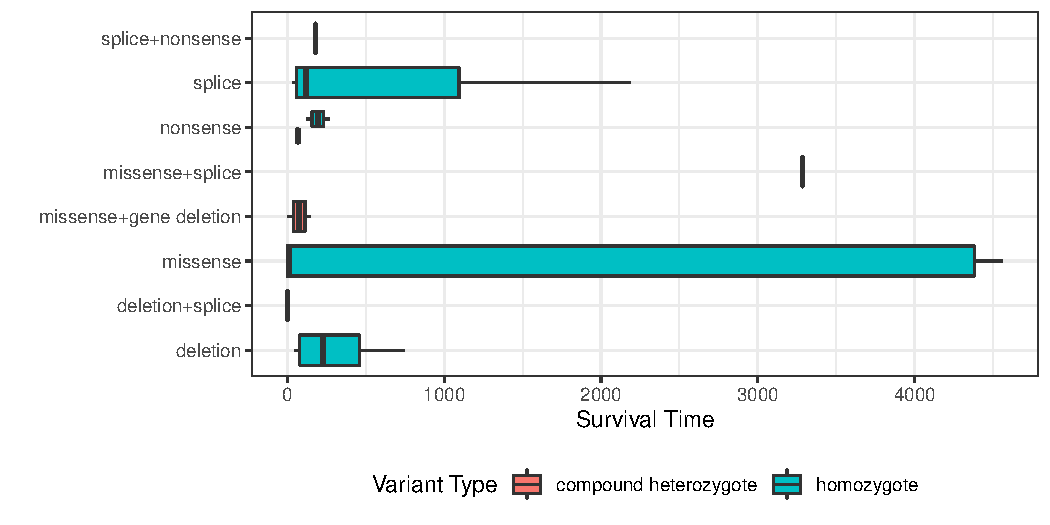
\includegraphics{paper_files/figure-pdf/unnamed-chunk-14-1.pdf}

A log-rank test was carried out to compare the survival curves of
patients stratified by the various gene variants and showed a
significant difference in the stratified survival curves
(\(\chi^2 = 14.8, p = 0.04)\) however due to the small sample size and
large number of possible variants, several had expected counts less than
5 which would create a violation in assumptions for the test.

\hypertarget{discussion}{%
\section{Discussion}\label{discussion}}

Often, data collected in studies is fit for descriptive purposes but not
for in-depth statistical analysis. This meta-review of current studies
was able to consolidate and make publicly available, data sets that
allow analysis to be conducted on emerging conditions such as NEDMABA.

The use of dimension reduction techniques were shown to be successful in
uncovering relevant and novel substructure in the data. This was
particularly evident with the detection of the accepted typical
phenotype of microcephaly, hypomyelination, arthrogryposis, simplified
gyral pattern and developmental delay.

After excluding two outlying remarkable cases, this analysis clearly
identifies the presence of an adjacent cluster of related features that
are not as well described in The Human Phenotype Ontology
\citep{kohler2021human} as shown in Table~\ref{tbl-hpo}. We identify the
prolific feature of `respiratory distress' as an expression more
commonly associated with \emph{other} features such as vocal cord palsy,
tracheostomy, tube feeding and Gastroesophageal reflux disease (GERD).
These features are present in the case reported data, but not well
described in HPO and help account for the variation seen in the clinical
phenotype in the first few principal dimensions.

Other smaller clusters identify outlying features that are expressed in
individuals or specific families. Many of the outlying features are
highly specific facial or anatomical dysmorphisms. While coarse facial
features are a noted and core presentation, those with a milder course
had clinical reports that articulated these dysmorphisms in much more
detail, which skewed the interpretation.

On a similar note, talipes appears as an isolated feature without the
typical microcephaly and hypomyelination. However, there was significant
heterogeneity in how feet contractures were reported in clinical case
reports. While distinctions were made during data pre-processing between
rocker-bottom feed and talipes, this likely to make intpretation
somewhat difficult. This is particularly clear as rocker-bottom feet was
found closely related in our analysis to other core features despite the
prevalence in HPO being quite low (2/21), suggesting possible
under-reporting or confounded reporting of this feature.

Another feature clusted within core identified features is bilateral
cleft lip. This condition has a reported frequency of just 2/21
(Table~\ref{tbl-hpo}) and may be an emerging feature for a more typical
presentation given its close relationship with other classic features.

The heterogeneous variation in the data was clearly evident however,
with the first four principal axes being required to explain more than
50\% of the variation in the data set. Visual inspection of the data
projected into this lower dimensional space indicate the primary sources
of variation in the clinical phenotype are explained by a few
individuals with very different clinical features. This has confounded
the typical or classical presentation. Not all features in the data were
included in this analysis, particular if isolated to just one case. In
this circumstance, these terms in Table~\ref{tbl-hpo} have been labelled
as `Isolated'.

While the number of clusters chosen all represent valid partition of the
data, some metrics indicated an optimal selection of 2 clusters. This
type of partition is useful when segregating outliers from the rest of
the data and is valid in some applications. In this study, a larger
number (5) was selected to align the goals of the analysis which was to
uncover distinct groups of features.

In terms of patient survival, the first few months show a sharp decline
in survival probability confirming early demise in the infant period as
a key factor. A small number of cases show much longer survival into
childhood and in some cases into the second decade of life. This work
identifies a one year survival rate of 0.403 (95\% CI: 0.252, 0.644). On
the other hand, a naive estimate using just the number of deceased
patients at this time as proportion of the study population is 0.57
(16/28). This highlights the importance of applying a survival analysis
technique that incorporates censoring so as not to erroneously
overestimate the survival probability. The current literature suggests
the type of gene variant has an impact on survival time, which seems to
be supported in this work. Through a comparison of multiple survival
curves, stratified by variation type, the limited sample size prevented
definitive conclusions with many cells having expected counts less than
5.

Despite NEDMABA exhibiting a diverse and heterogeneous clinical
phenotype, our analysis was able to identify meaningful substructures in
this data through the use of dimension reduction techniques (MCA) and
cluster analysis. This has isolated the classic NEDMABA phenotype of
microcephaly, hypomyelination, arthrogryposis, simplified gyral pattern
and developmental delay. Furthermore it has isolated additional distinct
groupings of features that are exhibited in patients such as vocal cord
paralysis, swallowing dysfunction, tube feeding and GERD. Furthermore,
we were able to quantify the expected baseline survival probabilities
for children with this condition as well as quantifying the significant
variation in these estimates. Future work is required with the benefit
of more cases, to better understand the differences in survival curves
for other factors associated with genotype.

\newpage

\hypertarget{appendix}{%
\section{Appendix}\label{appendix}}

\hypertarget{tbl-hpo}{}
\setlength{\LTpost}{0mm}
\begin{longtable}{llrl}
\caption{\label{tbl-hpo}A mapping table of phenotype terms from The Human Phenotype Ontology
(HPO) with clusters defined in this analysis. Not all clinical features
defined in the analysis are present in the HPO terms }\tabularnewline

\toprule
\multicolumn{3}{c}{HPO Data} & Derived Clusters \\ 
\cmidrule(lr){1-3} \cmidrule(lr){4-4}
HPO Term Name & Category & Frequency & \textbf{Cluster}\textsuperscript{1} \\ 
\midrule
Adducted thumb & Limbs & 1/21 & Isolated \\ 
Simplified gyral pattern & Nervous System & 12/18 & Core \\ 
Hypertonia & Musculature & 9/15 & Core \\ 
Seizure & Nervous System & 10/17 & Core \\ 
Hypotonia & Musculature & 4/15 & Core \\ 
Global developmental delay & Nervous System & 7/7 & Core \\ 
Highly arched eyebrow & Skin, Hair, and Nails & 2/21 & Isolated \\ 
Cerebellar hypoplasia & Nervous System & 10/21 & Core \\ 
Neonatal respiratory distress & Respiratory System & 14/17 & Adjacent \\ 
Bifid uvula & Head and neck & 1/21 & Isolated \\ 
Deep philtrum & Head and neck & 1/21 & Isolated \\ 
CNS hypomyelination & Nervous System & 7/19 & Core \\ 
Lumbar hypertrichosis & Skin, Hair, and Nails & 1/21 & Isolated \\ 
Birth length less than 3rd percentile & Growth & 6/11 & Core \\ 
Hypoplasia of the brainstem & Nervous System & 3/20 & Isolated \\ 
Tented upper lip vermilion & Head and neck & 3/21 & Isolated \\ 
Hypotelorism & Eye & 1/21 & Isolated \\ 
Short palpebral fissure & Head and neck & 4/21 & Outlying \\ 
Bilateral cleft lip & Head and neck & 2/21 & Core \\ 
Diabetes mellitus & Endocrine & 2/19 & Isolated \\ 
Single transverse palmar crease & Skin, Hair, and Nails & 1/21 & Isolated \\ 
Epicanthus & Head and neck & 5/21 & Outlying \\ 
Low anterior hairline & Head and neck & 2/21 & Outlying \\ 
Arthrogryposis multiplex congenita & Connective tissue & 17/20 & Core \\ 
Progressive microcephaly & Nervous System & 9/10 & Core \\ 
Microcephaly & Nervous System & 15/21 & Core \\ 
Thin upper lip vermilion & Head and neck & 2/21 & Outlying \\ 
Thin vermilion border & Head and neck & 3/21 & Isolated \\ 
Intrauterine growth retardation & Growth & 12/19 & Core \\ 
Posteriorly rotated ears & Ear & 2/21 & Adjacent \\ 
Narrow forehead & Head and neck & 1/21 & Isolated \\ 
Sloping forehead & Head and neck & 4/21 & Isolated \\ 
Smooth philtrum & Head and neck & 2/21 & Isolated \\ 
Short philtrum & Head and neck & 2/21 & Outlying \\ 
Premature birth & Prenatal and Birth & 7/18 & Core \\ 
Mandibular prognathia & Head and neck & 2/21 & Outlying \\ 
Wide intermamillary distance & Breast & 1/21 & Isolated \\ 
Depressed nasal bridge & Head and neck & 1/21 & Outlying \\ 
Downslanted palpebral fissures & Head and neck & 2/21 & Outlying \\ 
Short neck & Head and neck & 1/21 & Isolated \\ 
Bulbous nose & Head and neck & 2/21 & Isolated \\ 
Protruding ear & Ear & 2/21 & Outlying \\ 
Rocker bottom foot & Limbs & 2/21 & Core \\ 
\bottomrule
\end{longtable}
\begin{minipage}{\linewidth}
\textsuperscript{1}Clusters defined in this analysis mapped to HPO Terms\\
Source: The Human Phenotype Ontology (HPO) https://hpo.jax.org/app/browse/disease/OMIM:618622 \\
Reference: Köhler S, Gargano M, Matentzoglu N, Carmody LC, Lewis-Smith D, Vasilevsky NA, Danis D, Balagura G, Baynam G, Brower AM, Callahan TJ, Chute CG, Est JL, Galer PD, Ganesan S, Griese M, Haimel M, Pazmandi J, Hanauer M, Harris NL, Hartnett MJ, Hastreiter M, Hauck F, He Y, Jeske T, Kearney H, Kindle G, Klein C, Knoflach K, Krause R, Lagorce D, McMurry JA, Miller JA, Munoz-Torres MC, Peters RL, Rapp CK, Rath AM, Rind SA, Rosenberg AZ, Segal MM, Seidel MG, Smedley D, Talmy T, Thomas Y, Wiafe SA, Xian J, Yüksel Z, Helbig I, Mungall CJ, Haendel MA, Robinson PN. \emph{The Human Phenotype Ontology in 2021.} Nucleic Acids Res. 2021 Jan 8;49(D1):D1207-D1217. doi: {10.1093/nar/gkaa1043}. PMID: 33264411; PMCID: PMC7778952.\\
\end{minipage}

\hypertarget{tbl-profile}{}
\begin{longtable}[]{@{}rl@{}}
\caption{\label{tbl-profile}Assignment of clinical features with their
cluster. These clusters represent similar features projected onto the
first four MCA principal axes. Clusters that are on opposing sides of an
axes contract with each other and account for the largest amount of
variation in the data.}\tabularnewline
\toprule()
cluster & variable \\
\midrule()
\endfirsthead
\toprule()
cluster & variable \\
\midrule()
\endhead
1 & polyhydramnios \\
1 & short\_palpebral\_fissures \\
1 & patent\_ductus\_arteriosus \\
1 & thin\_lips \\
1 & prognathism \\
1 & pectus\_excavatum \\
1 & respiratory\_infections \\
2 & vocal\_cord\_palsy \\
2 & respiratory\_distress \\
2 & tracheostomy \\
2 & posteriorly\_angulated\_ears \\
2 & upper\_lip\_dysmorph \\
2 & tube\_feed \\
2 & gerd \\
2 & decreased\_craniofacial\_ratio \\
2 & short\_upturned\_nose \\
2 & borderline\_small\_brainstem \\
2 & enlarged\_ventricles \\
3 & epicanthal\_folds \\
3 & receding\_forehead \\
3 & spastic\_tetraparesis \\
3 & intubation \\
3 & low\_anterior\_hairline \\
3 & short\_philtrum \\
3 & hirsutism \\
4 & microcephaly \\
4 & sgp \\
4 & iugr \\
4 & talipes \\
4 & rocker\_bottom\_feet \\
4 & contractures\_hands\_deform \\
4 & arthrogryposis\_contractures\_other \\
4 & cleft\_lip \\
4 & coarse\_facial\_features \\
4 & hypomyelination \\
4 & cerebellar\_hypoplasia \\
4 & small\_anterior\_fontanel \\
4 & thin\_corpus\_collosum \\
4 & feeding\_swallow\_dysfxn \\
4 & hearing \\
4 & seizure \\
4 & agenesis\_of\_corpus\_callosum \\
4 & severe\_developmental\_delay \\
4 & at\_birth\_sga \\
4 & lissencephaly\_and\_cerebellar\_hypoplasia \\
4 & eeg\_normal \\
5 & hypercapnia \\
5 & inspiratory\_stridor \\
5 & oligohydramnios \\
5 & prominent\_ears \\
5 & dysmorphic\_features \\
5 & tracheo\_laryngomalacia \\
\bottomrule()
\end{longtable}

\hypertarget{tbl-dict}{}
\begin{longtable}{ll}
\caption{\label{tbl-dict}Data dictionary of the final data set used for the analysis. This
combines the case reports and supplied data for available and references
studies. The data has been transformed into a tidy format with
formatting applied. }\tabularnewline

\toprule
variable & type \\ 
\midrule
study & character \\ 
id & character \\ 
family & character \\ 
individual & factor \\ 
deceased & logical \\ 
survival\_time & numeric \\ 
variant\_type & factor \\ 
locus\_1 & numeric \\ 
locus\_2 & numeric \\ 
gender & factor \\ 
ethnicity & character \\ 
consanguineous & logical \\ 
termination & logical \\ 
birth\_gestation & numeric \\ 
route\_vaginal\_vs\_c\_sect & factor \\ 
birth\_weight & numeric \\ 
birth\_ofc & numeric \\ 
birth\_length & numeric \\ 
age\_at\_demise & numeric \\ 
age\_at\_last\_follow\_up & numeric \\ 
microcephaly\_ind & factor \\ 
sgp\_ind & factor \\ 
iugr\_ind & factor \\ 
talipes\_ind & factor \\ 
rocker\_bottom\_feet\_ind & factor \\ 
contractures\_hands\_deform\_ind & factor \\ 
vocal\_cord\_palsy\_ind & factor \\ 
arthrogryposis\_contractures\_other\_ind & factor \\ 
hypercapnia\_ind & factor \\ 
cleft\_lip\_ind & factor \\ 
inspiratory\_stridor\_ind & factor \\ 
polyhydramnios\_ind & factor \\ 
coarse\_facial\_features\_ind & factor \\ 
oligohydramnios\_ind & factor \\ 
respiratory\_distress\_ind & factor \\ 
tracheostomy\_ind & factor \\ 
prominent\_ears\_ind & factor \\ 
posteriorly\_angulated\_ears\_ind & factor \\ 
prominent\_philtrum\_ind & factor \\ 
upper\_lip\_dysmorph\_ind & factor \\ 
hypomyelination\_ind & factor \\ 
cerebellar\_hypoplasia\_ind & factor \\ 
short\_palpebral\_fissures\_ind & factor \\ 
epicanthal\_folds\_ind & factor \\ 
tube\_feed\_ind & factor \\ 
dysmorphic\_features\_ind & factor \\ 
patent\_ductus\_arteriosus\_ind & factor \\ 
small\_anterior\_fontanel\_ind & factor \\ 
receding\_forehead\_ind & factor \\ 
tracheo\_laryngomalacia\_ind & factor \\ 
gerd\_ind & factor \\ 
thin\_corpus\_collosum\_ind & factor \\ 
feeding\_swallow\_dysfxn\_ind & factor \\ 
seizures\_age\_started & character \\ 
seizure\_type\_s & character \\ 
eeg & character \\ 
sleeping\_problem & character \\ 
behavioral\_issues & character \\ 
skeletal\_changes\_scoliosis & numeric \\ 
hip\_luxation & numeric \\ 
development\_head\_control & character \\ 
sitting\_unsupported & character \\ 
crawling & character \\ 
walking & character \\ 
speech & character \\ 
iq\_int\_disability & character \\ 
cp & character \\ 
performance & character \\ 
neuro\_exam\_eye\_mvts\_nystagmus & character \\ 
strabismus & character \\ 
feeding\_swallow\_dysfxn & character \\ 
gag & character \\ 
tone & character \\ 
strength & character \\ 
sensory\_deficits & character \\ 
abnormal\_mvts & character \\ 
dtr & character \\ 
other\_neuro\_signs & character \\ 
sensory\_vision & character \\ 
hearing & character \\ 
other\_organs & character \\ 
endocrinology & character \\ 
functional\_tests & character \\ 
metabolic\_investigation & character \\ 
cardiology & character \\ 
seizure & numeric \\ 
agenesis\_of\_corpus\_callosum & factor \\ 
abnormal\_pattern\_of\_cerebral\_sulci & factor \\ 
left\_sided\_gallbladder & factor \\ 
suspected\_brain\_stem\_dysfunction & factor \\ 
spastic\_tetraparesis & factor \\ 
severe\_developmental\_delay & factor \\ 
acidosis & factor \\ 
small\_thorax & factor \\ 
cyanosis & factor \\ 
intubation & factor \\ 
apnea & factor \\ 
mr\_is\_reportedly\_with\_migrational\_defect & factor \\ 
at\_birth\_sga & factor \\ 
epilepsy\_and\_apnea & factor \\ 
choanal\_atresia\_surgeries\_for\_transposition\_of\_the\_great\_arteries & factor \\ 
interventricular\_and\_interatrial\_defects & factor \\ 
smooth\_philtrum & factor \\ 
thin\_lips & factor \\ 
bilateral\_simian\_creases & factor \\ 
low\_anterior\_hairline & factor \\ 
short\_philtrum & factor \\ 
prominent\_nose\_bridge & factor \\ 
depressed\_nasal\_bridge & factor \\ 
prominent\_suture\_ridges & factor \\ 
hypotelorism & factor \\ 
hypertrichosis\_of\_lower\_back & factor \\ 
decreased\_craniofacial\_ratio & factor \\ 
there\_is\_overlapping\_of\_the\_sutures & factor \\ 
bitemporal\_narrowing & factor \\ 
short\_upturned\_nose & factor \\ 
short\_neck & factor \\ 
upward\_sweep\_of\_hair & factor \\ 
arched\_eye\_brows & factor \\ 
bulbous\_nose & factor \\ 
prominent\_lower\_lip & factor \\ 
broad\_chin & factor \\ 
prognathism & factor \\ 
asd & factor \\ 
left\_multicystic\_dysplastic\_kidney & factor \\ 
anteriorly\_placed\_anus & factor \\ 
dilated\_cardiomyopathy & factor \\ 
cryptorchidism & factor \\ 
hirsutism & factor \\ 
intestinal\_malrotation & factor \\ 
dysphagia & factor \\ 
intermittent\_sinus\_bradycardia & factor \\ 
bilateral\_staphylomas & factor \\ 
lissencephaly & factor \\ 
echogenic\_choroid\_plexus\_on\_head\_us & factor \\ 
head\_us\_mild\_ventriculomegaly & factor \\ 
brain\_parenchyma\_appears\_homogeneous\_without\_evidence\_of\_focal\_lesion & factor \\ 
hypoplastic\_cerebellum & factor \\ 
borderline\_small\_brainstem & factor \\ 
abnormal\_cerebellar\_folia & factor \\ 
mild\_vermian\_hypoplasia & factor \\ 
asymmetry\_of\_lateral\_ventricles & factor \\ 
lissencephaly\_and\_cerebellar\_hypoplasia & factor \\ 
signs\_of\_hypoxic\_encephalopathy & factor \\ 
mild\_dilation\_of\_virchow\_robins\_spaces & factor \\ 
pectus\_excavatum & factor \\ 
widely\_spaced\_nipples & factor \\ 
respiratory\_infections & factor \\ 
enlarged\_ventricles & factor \\ 
eeg\_normal & numeric \\ 
bifid\_uvula & factor \\ 
under\_developed\_cerebellar\_inferior\_vermis & factor \\ 
\bottomrule
\end{longtable}

\newpage


\renewcommand\refname{References}
  \bibliography{bibliography.bib}


\end{document}
